% 03_hw

\subsection{Quantenmechanische Betrachtung}

\begin{frame}
  \frametitle{Repetition Wasserstoffatom}
	\begin{columns}
		 \column{.5\textwidth}
			 \begin{itemize} 
			\item[]	$h\nu = \Delta E$ 
			\item[]   $h:$ Planksches  Wirkungsquantum
		 	\item[]   $\nu:$ Frequenz
		 	\item[]   $E: $ Energie
		 	\end{itemize}		 			 	
		\column{.5\textwidth}
		 	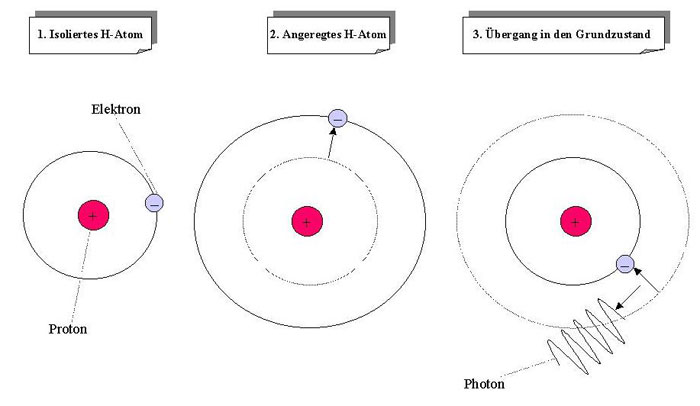
\includegraphics[width = 5cm]{./pictures/wasserstoffBohr}
		 	
			Spektrum Balmer-Serie
		 	
		 	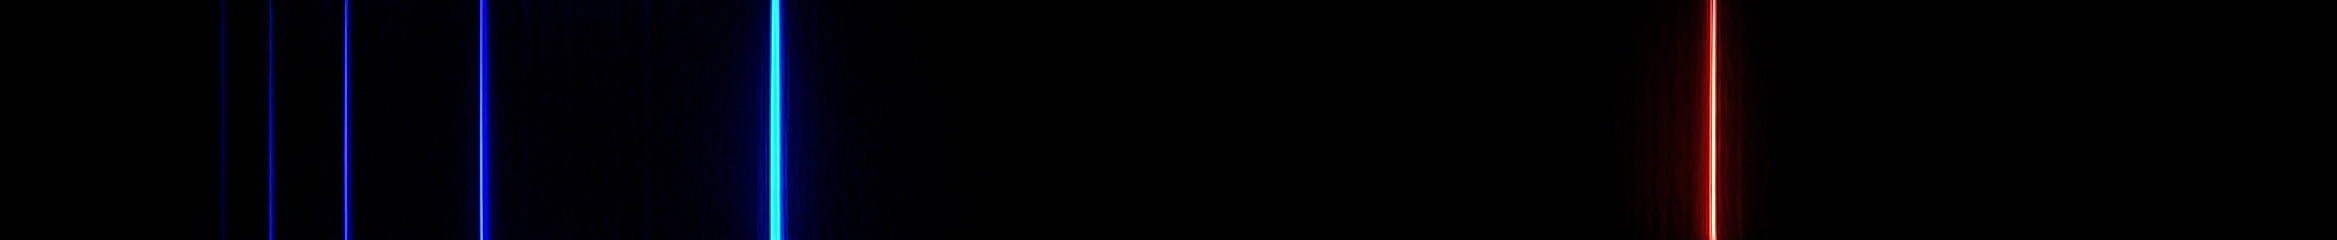
\includegraphics[width = 5cm]{./pictures/wasserstoffSpektrum}
	
	\end{columns}

\end{frame}

\begin{frame}
	\frametitle {Repetition Wasserstoffatom}
	\begin{center}
		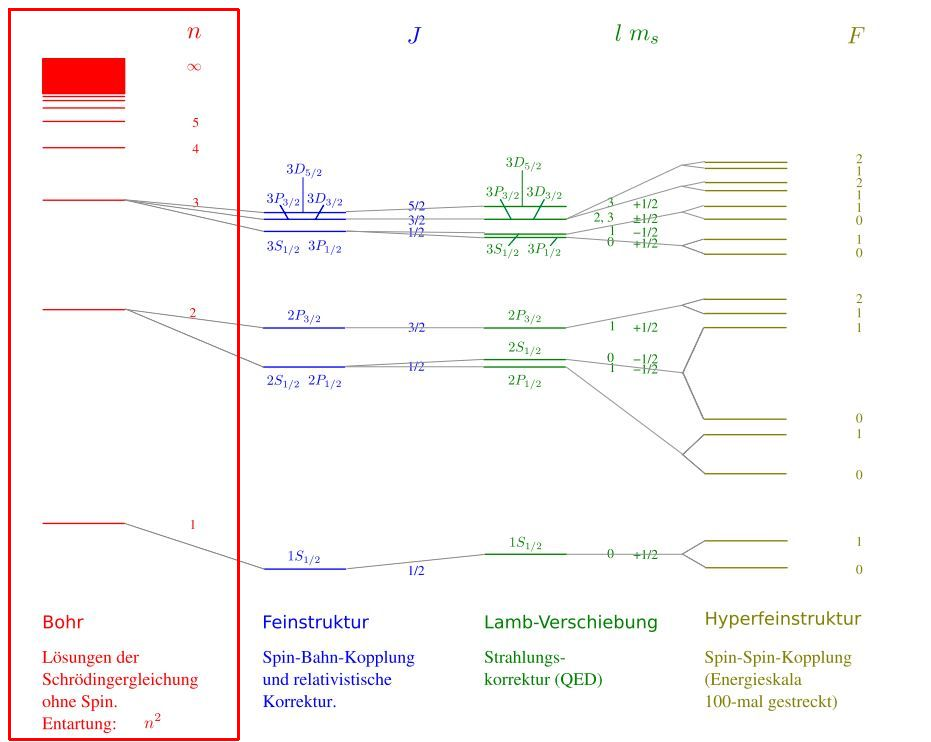
\includegraphics[width = 8cm]{./pictures/energieniveaus1}
	\end{center}

	
\end{frame}

\begin{frame}
	\frametitle{Repetition Wasserstoffatom}
	\begin{columns}
	\column{.5\textwidth}

	Übergang $H\alpha: 3 \rightarrow 2: \lambda_1 = 656.3nm$
		 	
		 	$\nu_1 = \dfrac{c}{\lambda_1} = 457.3 THz $
		 	\vspace{.5cm}
		 	
		 	Übergang $8 \rightarrow 2: \lambda_2 = 388.8nm$
		 	
		 	$\nu_2 = \dfrac{c}{\lambda_2} = 771.2 THz$
	\column{.5\textwidth}
	Spektrum Balmer-Serie
				
	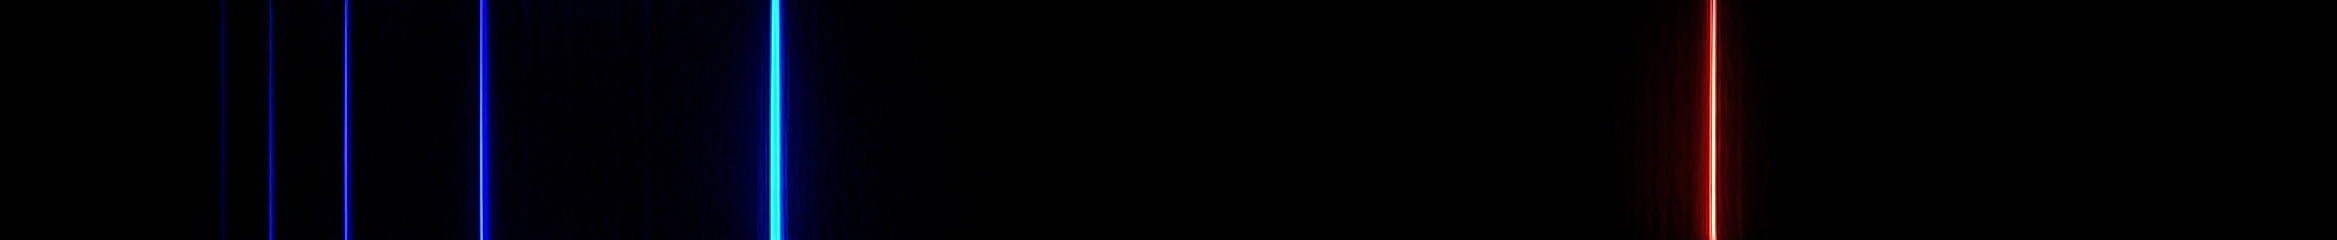
\includegraphics[width = 5cm]{./pictures/wasserstoffSpektrum}
				
	\end{columns}
\end{frame}


\begin{frame}
	\frametitle {Feinstrukturübergang}

	\begin{center}
		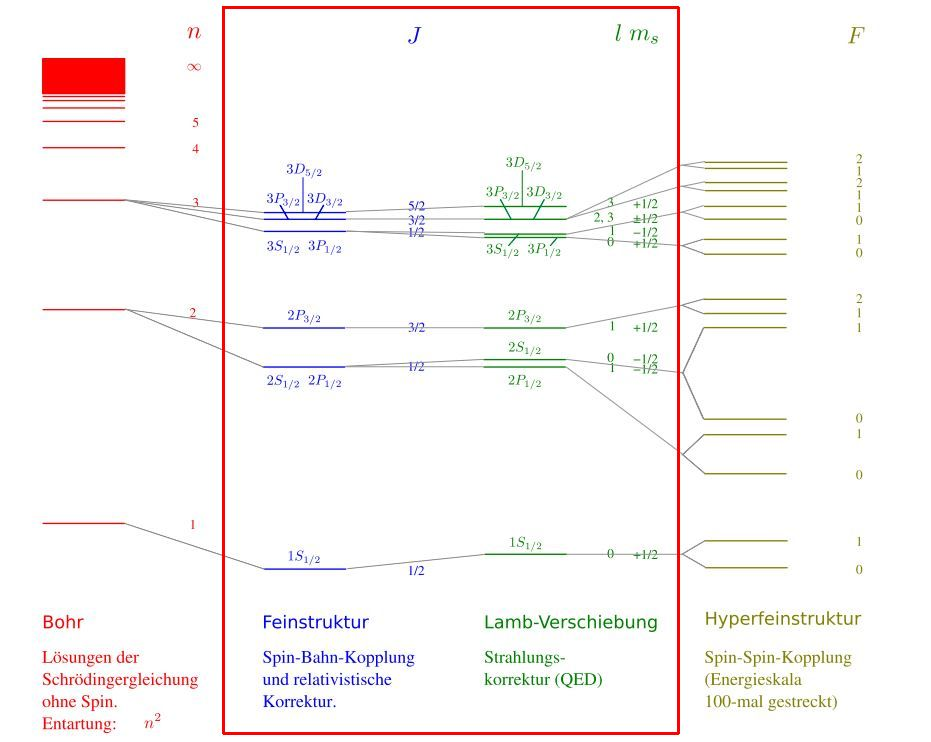
\includegraphics[width = 8cm]{./pictures/energieniveaus2}
	\end{center}
	
\end{frame}


\begin{frame}
  \frametitle{Feinstrukturübergang}
	\begin{columns}
		\column{.6\textwidth}
		\begin{itemize}
		\item[-] Beweis für Elektronenspin
		\item[-] Wechselwirkung zwischen Spin und Bahndrehimpuls
		\item[-] Störungstheorie
		\item[]  $H = H_0+W_M + W_{SB} +W_D+ \dots$
		\item[]  relativistische Korrektur, Spin-Bahn-Kopplung, Darwin-Term, ...
		\end{itemize}
		
		
		\column{.4\textwidth}
		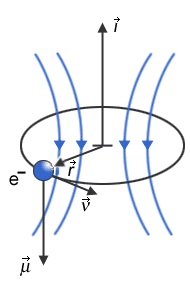
\includegraphics[width = 4cm]{./pictures/feinstrukturelektron}
			
	\end{columns}
	
	
	
\end{frame}

\begin{frame}
	\begin{columns}
		\column{.6\textwidth}
		Übergang $2P_{3/2} \rightarrow 2P_{1/2}: \lambda = 2.76cm$
				
		$\nu_1 = \dfrac{c}{\lambda_1} = 10,9 GHz $
		\vspace{.5cm}
				
		\column{.4\textwidth}
		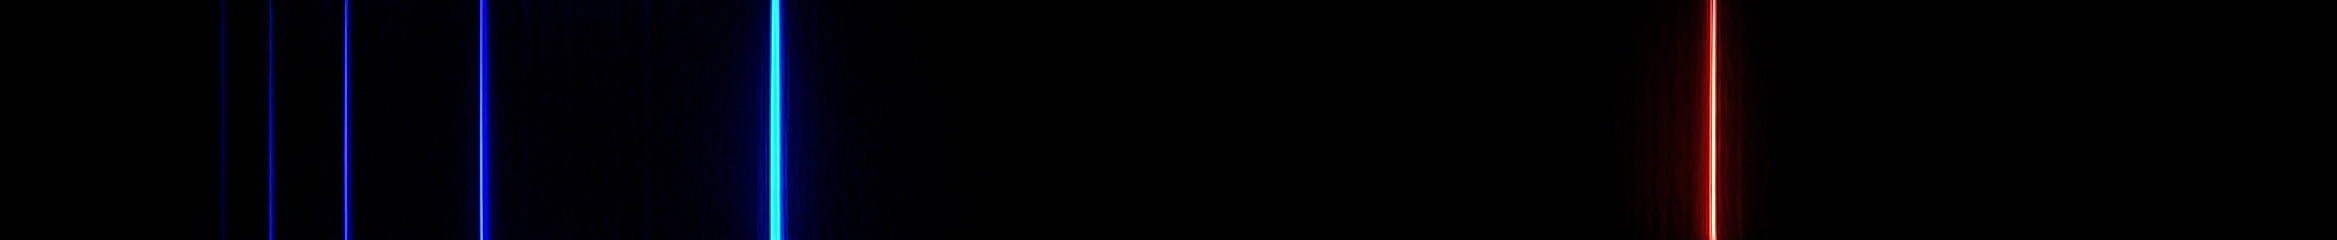
\includegraphics[width = 4cm]{./pictures/wasserstoffSpektrum}
			
		
\includegraphics[width = 4cm]{./pictures/fine_structure_hydrogen}
	\end{columns}
\end{frame}

\begin{frame}
	\frametitle {Feinstrukturübergang}
	
	\begin{center}
		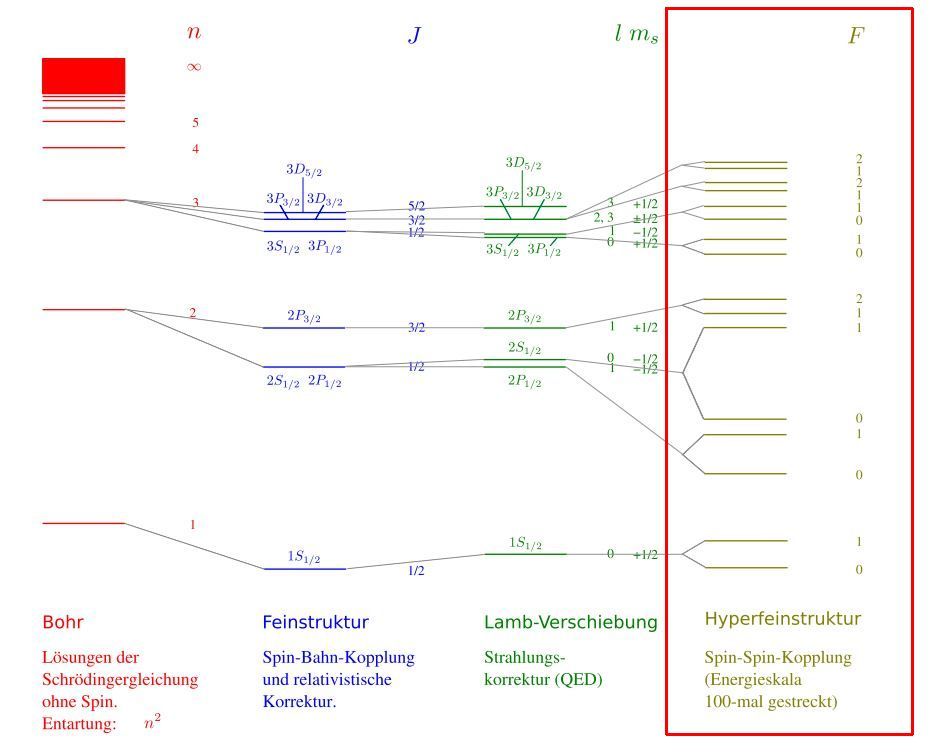
\includegraphics[width = 8cm]{./pictures/energieniveaus3}
	\end{center}
	
\end{frame}

\begin{frame}
	\frametitle{Hyperfeinstrukturübergang}
	\begin{columns}
		\column{.6\textwidth}		
		\begin{itemize}
			\item[-] Wechselwirkung Elektron $\leftrightarrow$ Kern
			\item[-] Energiezufuhr kann zu Spinwechsel des elektrons führen
			\item[ ]
			\item[-] 21cm, wichtig in der Astronimie
			\item[]
			\item[-] Rubidium, 6,834 GHz
		\end{itemize}
		\column{.4\textwidth}
		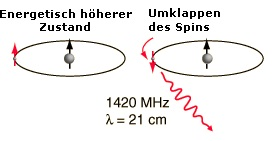
\includegraphics[width = 4cm]{./pictures/h21b}
	\end{columns}
	
\end{frame}

\begin{frame}
	\frametitle{Alkalimetalle}
	\begin{columns}
		\column{.6\textwidth}
		\begin{itemize}
			\item [-] abgeschlossene Schalen, 1 elektron
			\item [-] reaktionsfreudige Metalle
		\end{itemize}
		\column{.4\textwidth}
		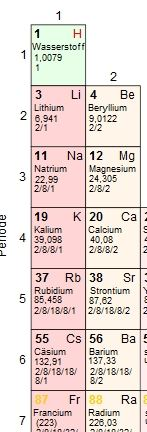
\includegraphics[width = 2cm]{./pictures/alkalimetalle}
	\end{columns}
\end{frame}


%%% Local Variables: 
%%% mode: latex
%%% TeX-master: "../main"
%%% End: 
